\chapter{The Social AR Continuum}
\label{ch:continuum}

% Mark: I think you still might need a one sentence explanation of what the Social AE Continuum is. It's a little unclear from what you've written here
This chapter describes The Social AR Continuum, a space for shared social experiences using wearable AR. It explores various dimensions, discusses options for each dimension, and outlines possible scenarios where these options might be useful. The Social AR Continuum is a set of dimensions that describe different ways of sharing the social experience through wearable AR devices. 

Mixed and Augmented Reality allows us to visualise information in place. This information can have a specific relationship with that place (e.g., textual labels providing additional information with respect to the place) but their relation can also be that the place is just a good "position" to visualise this information (e.g., a physical wall in a room being a good position to visualise/augment pictorial information that has otherwise no immediate connection to this wall). In particular, the latter can also be used to visualise information created within the social networks of the user. This is of relevance because social networks (private and professional) are nowadays probably one of the most significant data sources/content generators for digital information. Given the sheer amount of information, intuitive and useful visualisation of this information may support the user when AR interfaces are more ubiquitous. Special care has to be taken when visualising information, not only on where to place it but also on how to visualise the information. Besides the question of where to place the digital information, a key question is also how this information can be represented depending on the social proximity between the users and their social graph. This is the motivation for defining a continuum that identifies the main dimensions that can be manipulated when exploring the sharing of experiences and information using an AR interface. 


% Tobias: Again, this is just some sentences that just came out of my head. You can use or not use at your own risk and will. However, it has to be expanded (your story but also my draft above) as there is way more to say about. At occasions, you will have the feeling that you will repeat things that you mentioned earlier (e.g. introduction and related work). That is normal, and the repeating of information is often needed for the reader to follow your motivation and argumentation. Remember: Your reviewers are likely reading your thesis late after work and will be tired. An occasional reminder of what this is all about will be appreciated as long as it is coherent and you do not start to contradict yourself.

% This work aims to layout the space of the Social AR Continuum for social sharing experiences by looking at parameters and options that can be manipulated in terms of people, objects and interactions to create a shared social AR experience. Before diving into the parameters of shared social experiences, 
The next section explores potential future scenarios where people would want to share social experiences through AR.

\pagebreak
\section{Scenarios}
% \todo[inline]{explain all the things no just what is depicted in the picture…. later explain the other scenarios but similarly motivate for each scenario why this is a valid and important scenario.}

% Tobias: First of all I like graphics etc. I was even thinking if you should start with the scenarios before coming to the AR continuum. IIf you could use your scenarios to motivate the need for an AR continuum better?! Later, you can use them again to explain some of the dimensions. In any case, they are under-utilised at the moment. They need a better explanation and better integration. For example, I would not start with the decoration one because it is the weakest one in my opinion. Maybe better start with working from home and the social meeting. You could start with that  ….. blabla bla… explain all the things no just what is depicted in the picture…. later explain the other scenarios but similarly motivate for each scenario why this is a valid and essential scenario. 

% Again, these are all recommendations, and you can take it or leave it (or take parts of it). In any case, you need to integrate more references. I only put in the last part some examples on where they are needed, but basically, every big statement should be supported. I think this is all-important because when the reader is not buying in into your scenarios, you will have a hard time selling your conceptual solutions for each scenario. The reader will simply say: The scenario is not a real scenario or is to irrelevant to be addressed by a PhD thesis as it is not solving a real problem (current and future). This is a bit of the issue with the decoration scenario, which is a bit random. Keep it but do not put it first.

% Finally, please be more verbose in your figure captions. I have the tendency to be very long (see my PhD thesis and most of my papers) but really take the space to explain what is going on in the figure and do not only provide a "figure name". It is OK if parts are replicated in the body text. But the figure should work without the body text, and the body text should work without the figure caption.

% Let us consider the following future scenarios of sharing social AR experiences:

\subsection{Working from home}

There is increasing support for working from home \cite{Bloom2015, Crosbie2004, Olson1984} and AR/MR could be a key technology here to connect remote teams and people \cite{Koehne2012, Maarouf2012}. However, when sharing information with remote parties, we should also consider their social proximity when deciding on what to share and how to share it. Let us consider the following example where user A is working from home and is using an AR system to share. The user is working from home (Figure \ref{fig:illustration:group-meeting}) and sharing their surroundings with 1) a close colleague with a few messy objects hidden/blocked, 2) a colleague who sees a clean and tidy room with projection on the wall as additional augmentation, and 3) a group meeting with other workers where nothing is visible in the background. 

\begin{figure}[ht]
    \centering
    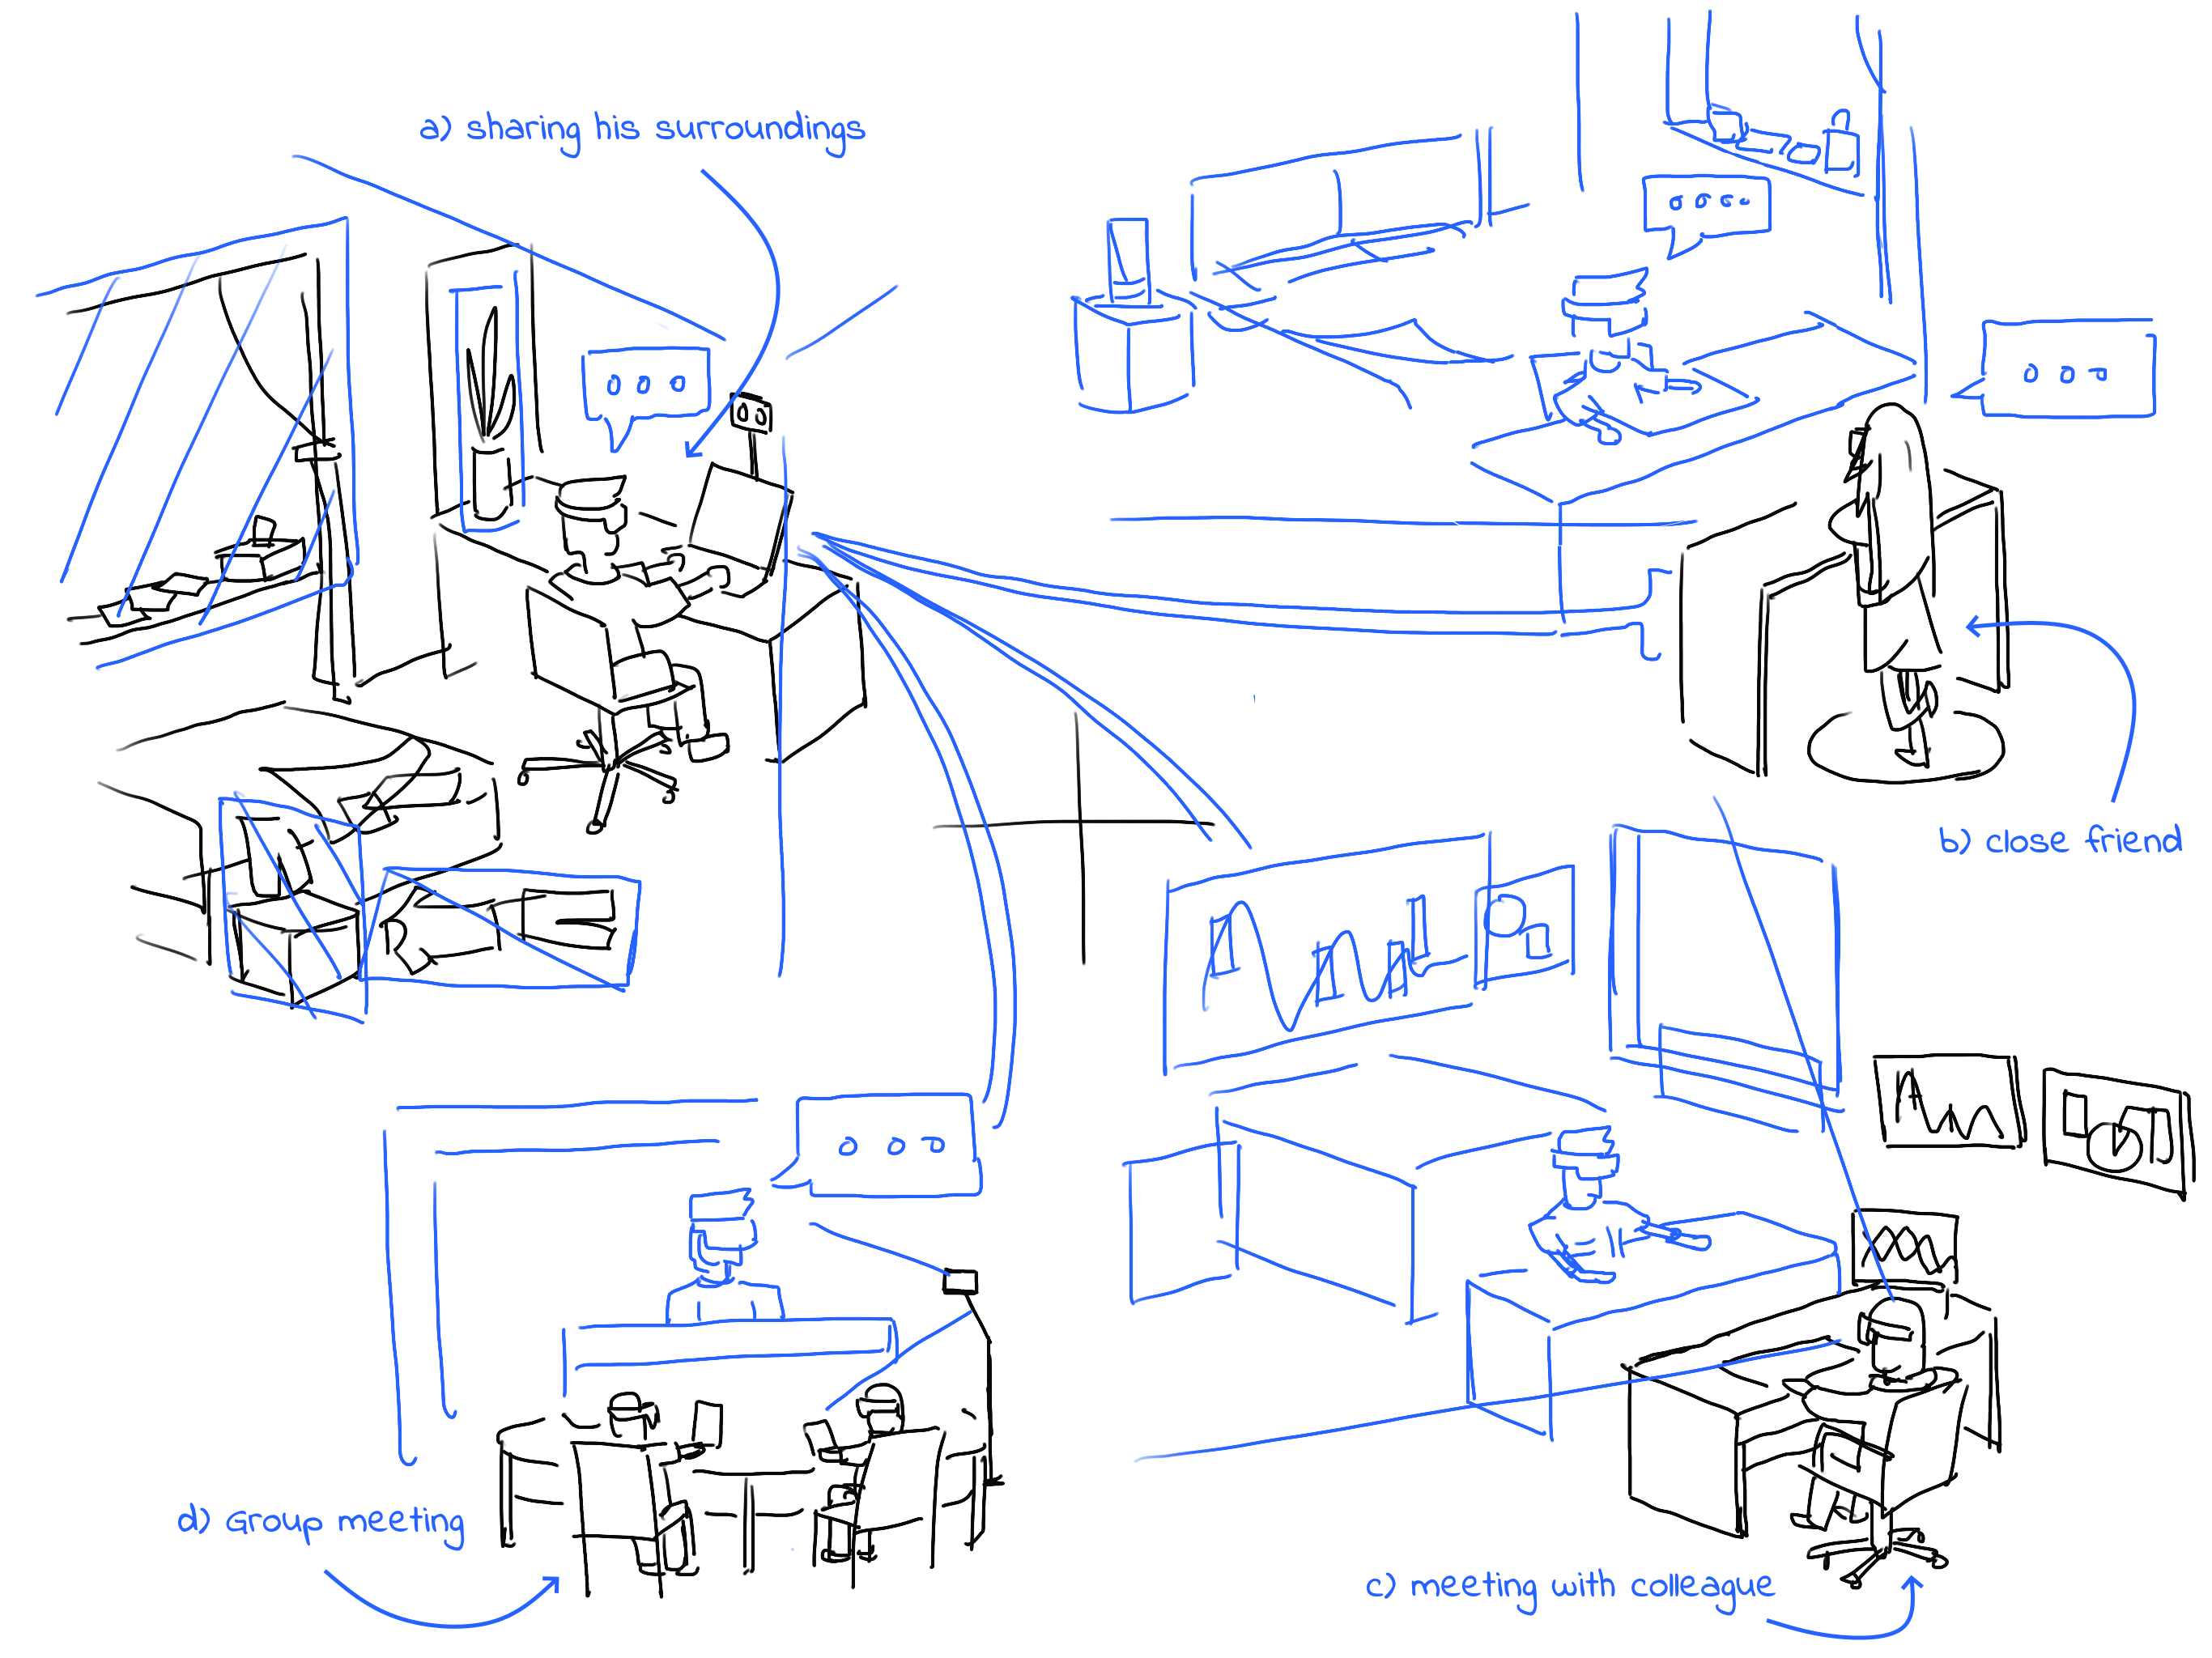
\includegraphics[width=\linewidth]{images/30-continuum/illustrations/2_Group_Meeting.png}
    \caption{Working from home scenario. The user (top left - [a]) is sharing his space with 3 different people; a friend (top right - [b]) where she sees his background space tidy, a co-worker (bottom right [c]) where most things in the background are overlaid with a box hiding the details, and a business group meeting (bottom left [d]) where nothing is visible from his background.
    (Illustrated by Kris Tong)}
    \label{fig:illustration:group-meeting}
\end{figure}

\pagebreak
\subsection{Conference}

The user is at a conference (Figure \ref{fig:illustration:conference}) and shares an idea that he is thinking about. However, because people around him are not close to him, they see low-fidelity details about these ideas (e.g., abstract and title). While networking with others, the user may choose to share more details about the idea with a particular person who is in a direct conversation with him and interested in further collaboration opportunities.

\begin{figure}[ht]
    \centering
    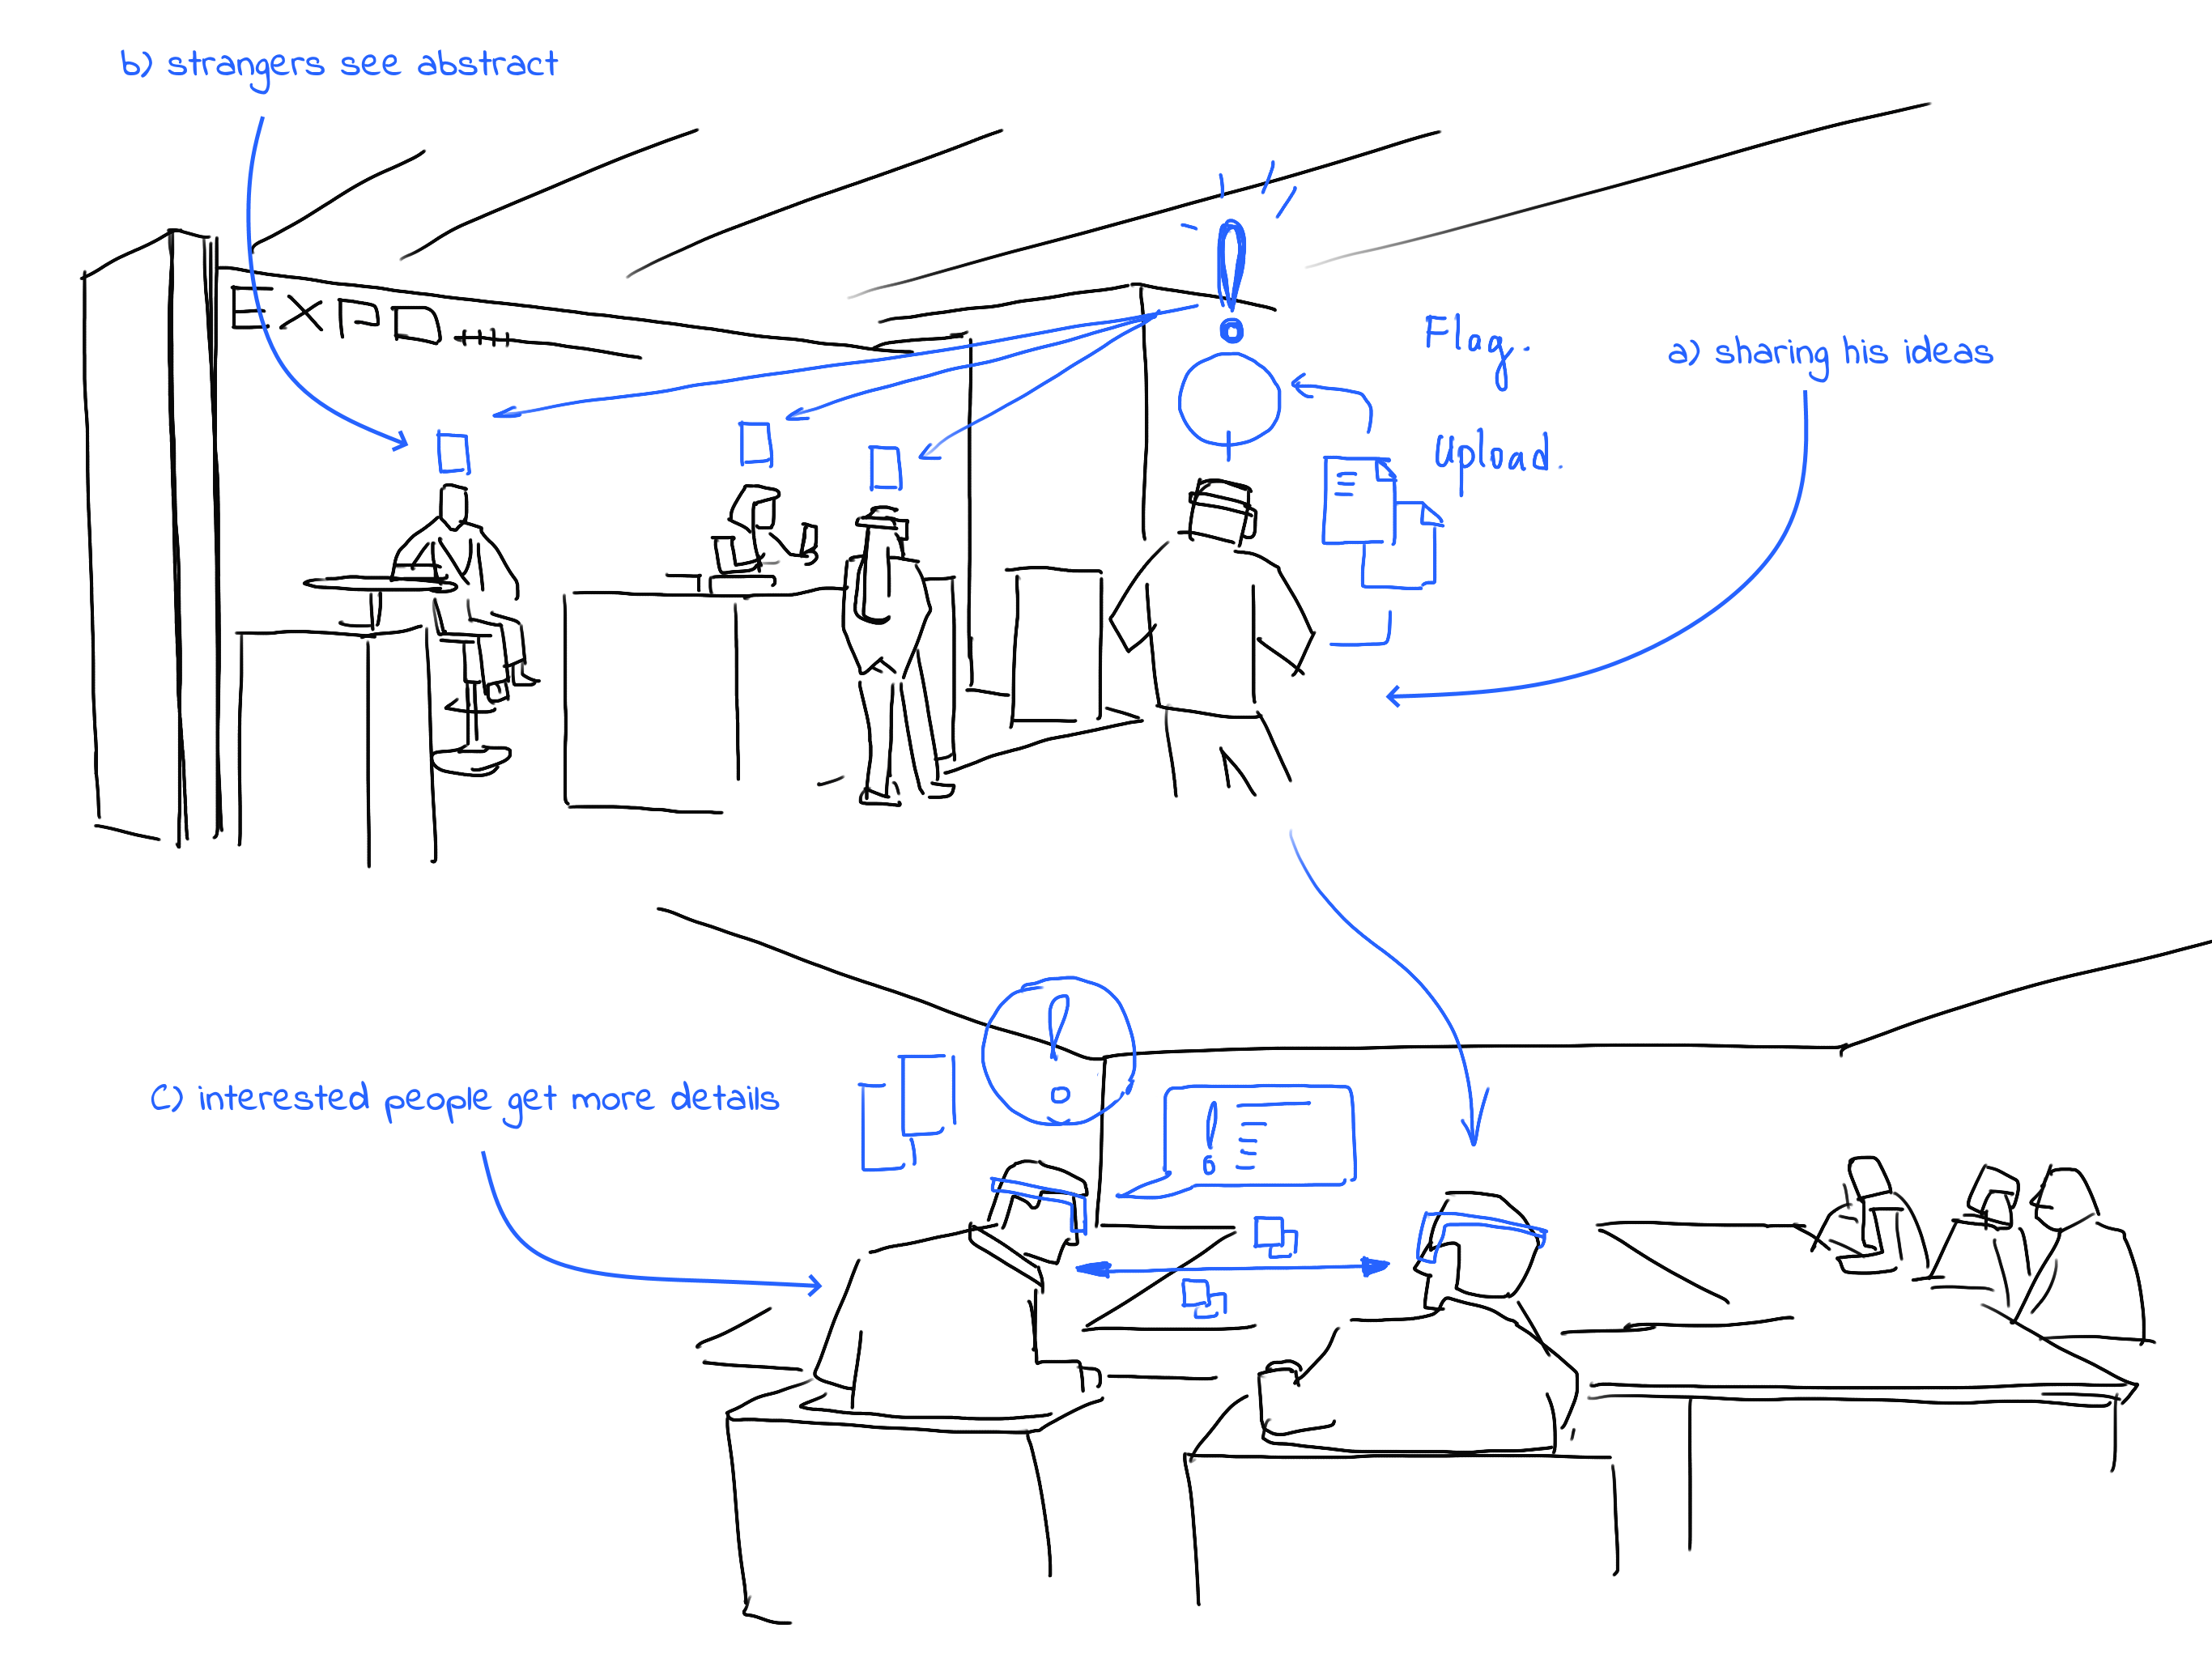
\includegraphics[width=\linewidth]{images/30-continuum/illustrations/4_Flag_On_Conference.png}
    \caption{Conference scenario. The user (top) walks through a conference sharing his ideas about the conference topic in high-level with strangers. When he meets a like-minded person (bottom), he may share more details about these ideas with that person. (Illustrated by Kris Tong)}
    \label{fig:illustration:conference}
\end{figure}

\pagebreak
\subsection{Social event}

The user is at a social event (Figure \ref{fig:illustration:social-event}), where he is meeting people face to face for a drink. He can see through their headset what their friends are sharing. For the close friends, he can see high-fidelity material such as 360-degree videos of their last trip, while for others who are less close to him, he sees low-fidelity media such as 2D images. 

\begin{figure}[ht]
    \centering
    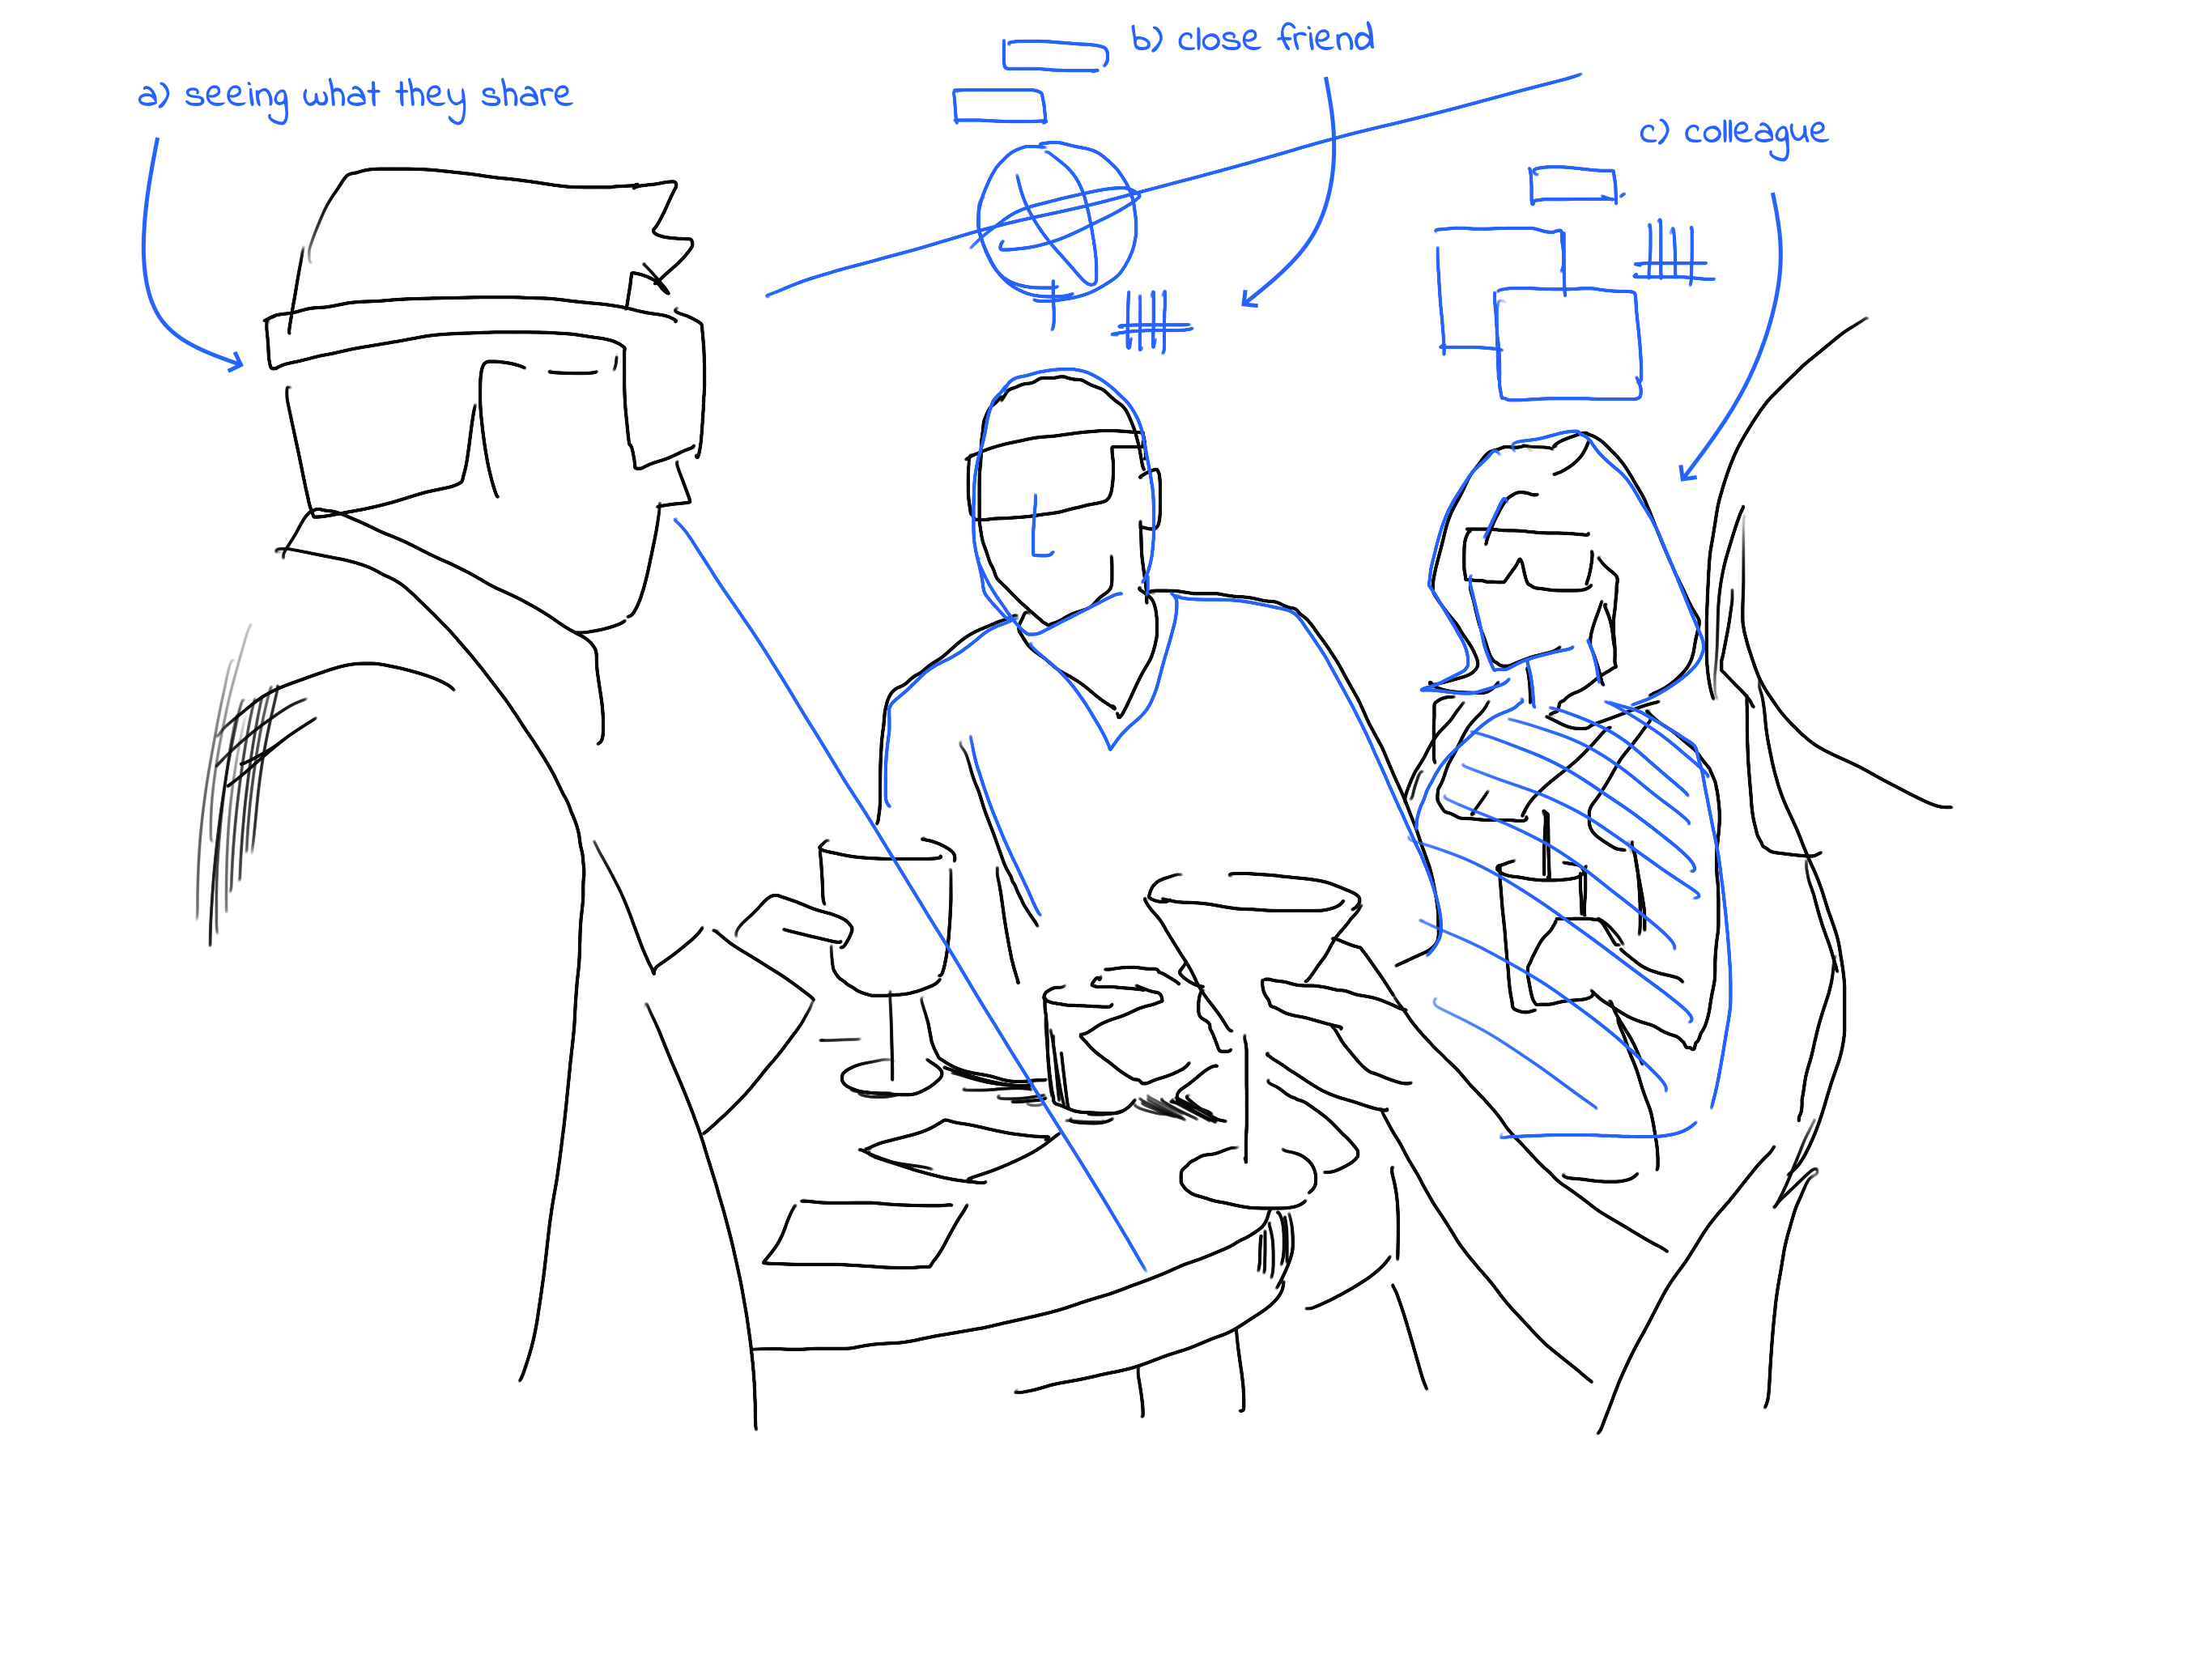
\includegraphics[width=\linewidth]{images/30-continuum/illustrations/3_Bar_Scene.png}
    \caption{Social event scenario. The user meets friends and colleagues face to face at a bar. He sees what they are sharing with him as images/video as AR floating on top of their heads. Based on how socially close with them, he sees more detail (higher fidelity) content from close friends than from strangers or colleagues.  (Illustrated by Kris Tong)}
    \label{fig:illustration:social-event}
\end{figure}

\pagebreak
\subsection{Collaborative decoration}
The user is sharing their room (Figure \ref{fig:illustration:remote-bed}) for decoration purposes with 1) a wife, 2) parents, and 3) a friend. The wife will see the full details of the room. The parents see most details, but a few items in the room are blocked/hidden. The friend will see an abstraction of the room with no details. 

\begin{figure}[ht]
    \centering
    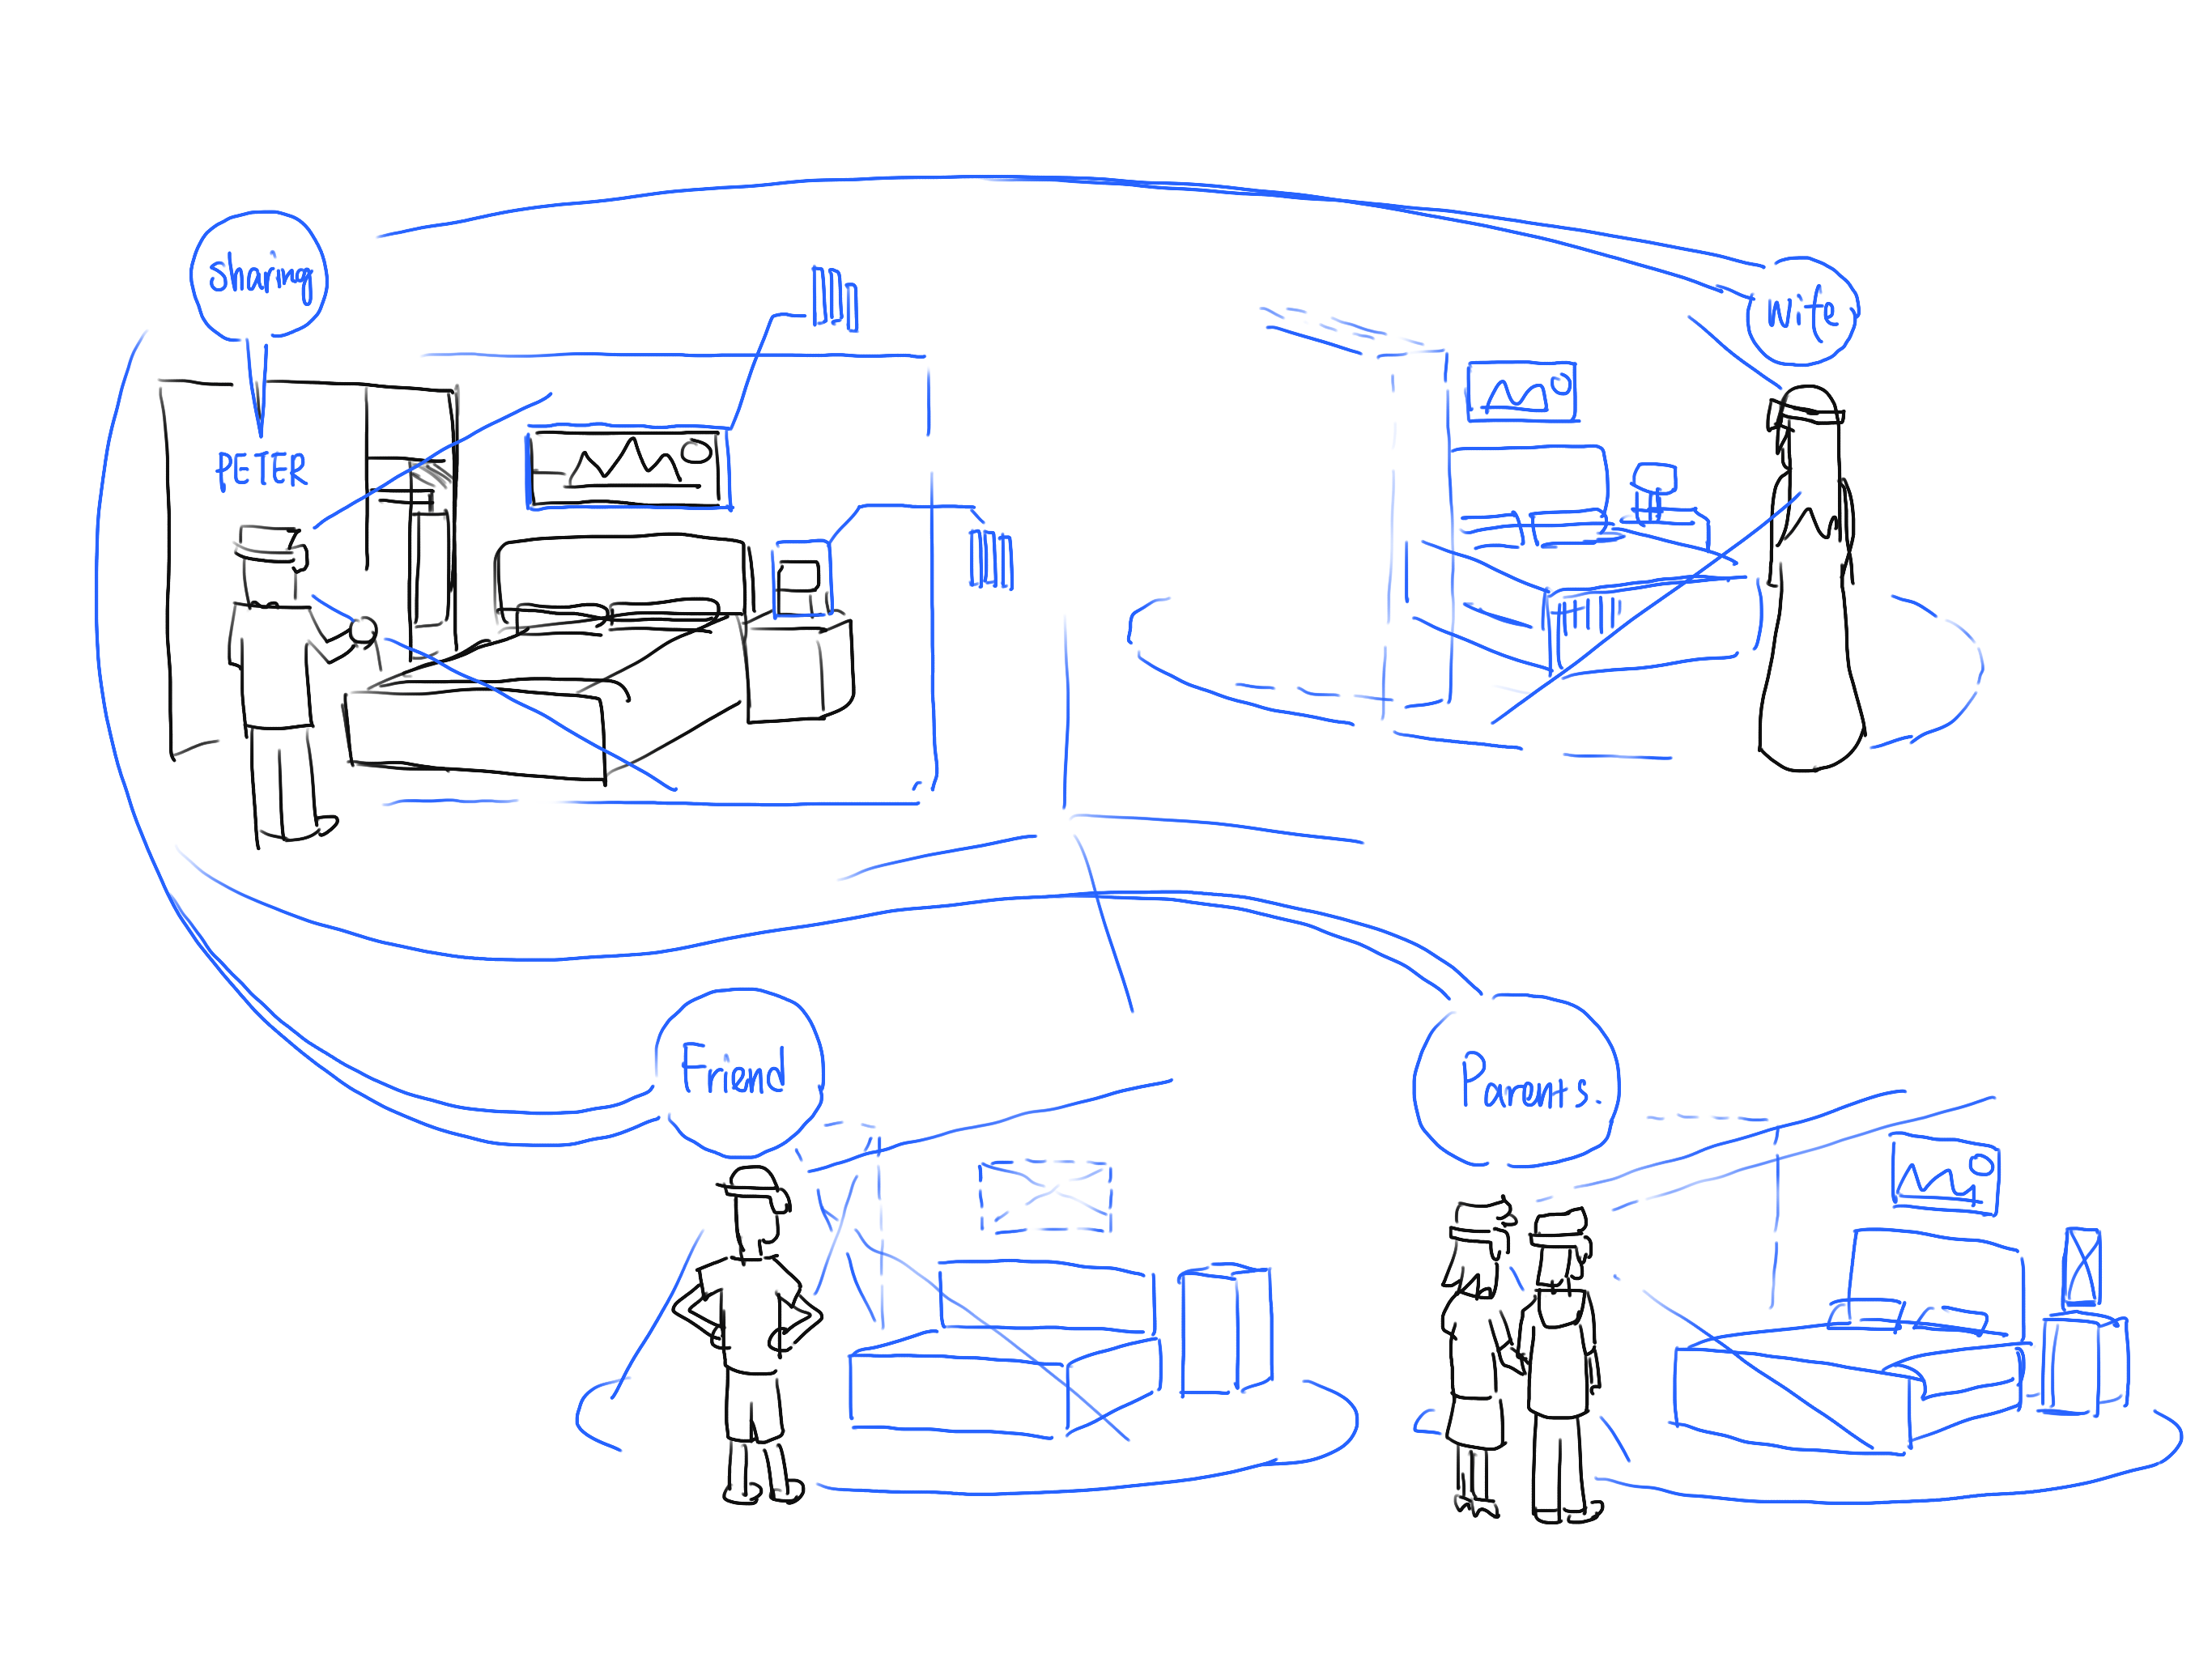
\includegraphics[width=\linewidth]{images/30-continuum/illustrations/1_Remote_Bed.png}
    \caption{Collaborative decoration scenario. The user (top left) shares a 3D scan of his bedroom and invites three people to join in virtually to give suggestions on decorating the room. His wife can see all details about the room and has access to change or add new decorations to the room. His parents can see fewer details about the room than the wife and can give new decoration of furniture items but not change anything in the room. His friend can see a more abstract version of the room and can only give suggestions as text comments.  (Illustrated by Kris Tong)}
    \label{fig:illustration:remote-bed}
\end{figure}

\pagebreak
\section{The Social AR Continuum Dimensions}
% \todo[inline]{ what inspirations? which papers (1/2 page)  initial axes, however realised}
% Tobias: How have you methodologically created the AR continuum: Once you made clear why you need this continuum, you need to also better explain how you have created it. It sounds at the moment a bit like, we need it, and here it is. But how have you created it? Brainstorming alone, with colleagues, any well know HCI approach? A brainstorming meeting with AR professionals could be the answer here but what has driven this brainstorming and what was the overarching idea. Why are certain metrics not in the continuum and could have looked differently? Do you have earlier versions that you can share and explain why they needed more work. I think if you can demonstrate the iterative development that the model underwent, it would support you. In any case you need to explain how you have designed it.

The scenarios of social AR experiences highlighted patterns in terms of how we see others and objects and how to interact with them. Using observations from previous user studies in virtual social networking, collaborative AR and inspiration from continuum designs, the concept of a continuum started to crystallise. A focus group study as part of this thesis (described in Section \ref{sec:contacts:visualising}) uncovered three main categories of parameters involved in social AR; 1) people, 2) objects \& data and 3) interactions (Figure \ref{fig:continuum:categories}).

\begin{figure}[ht]
    \centering
    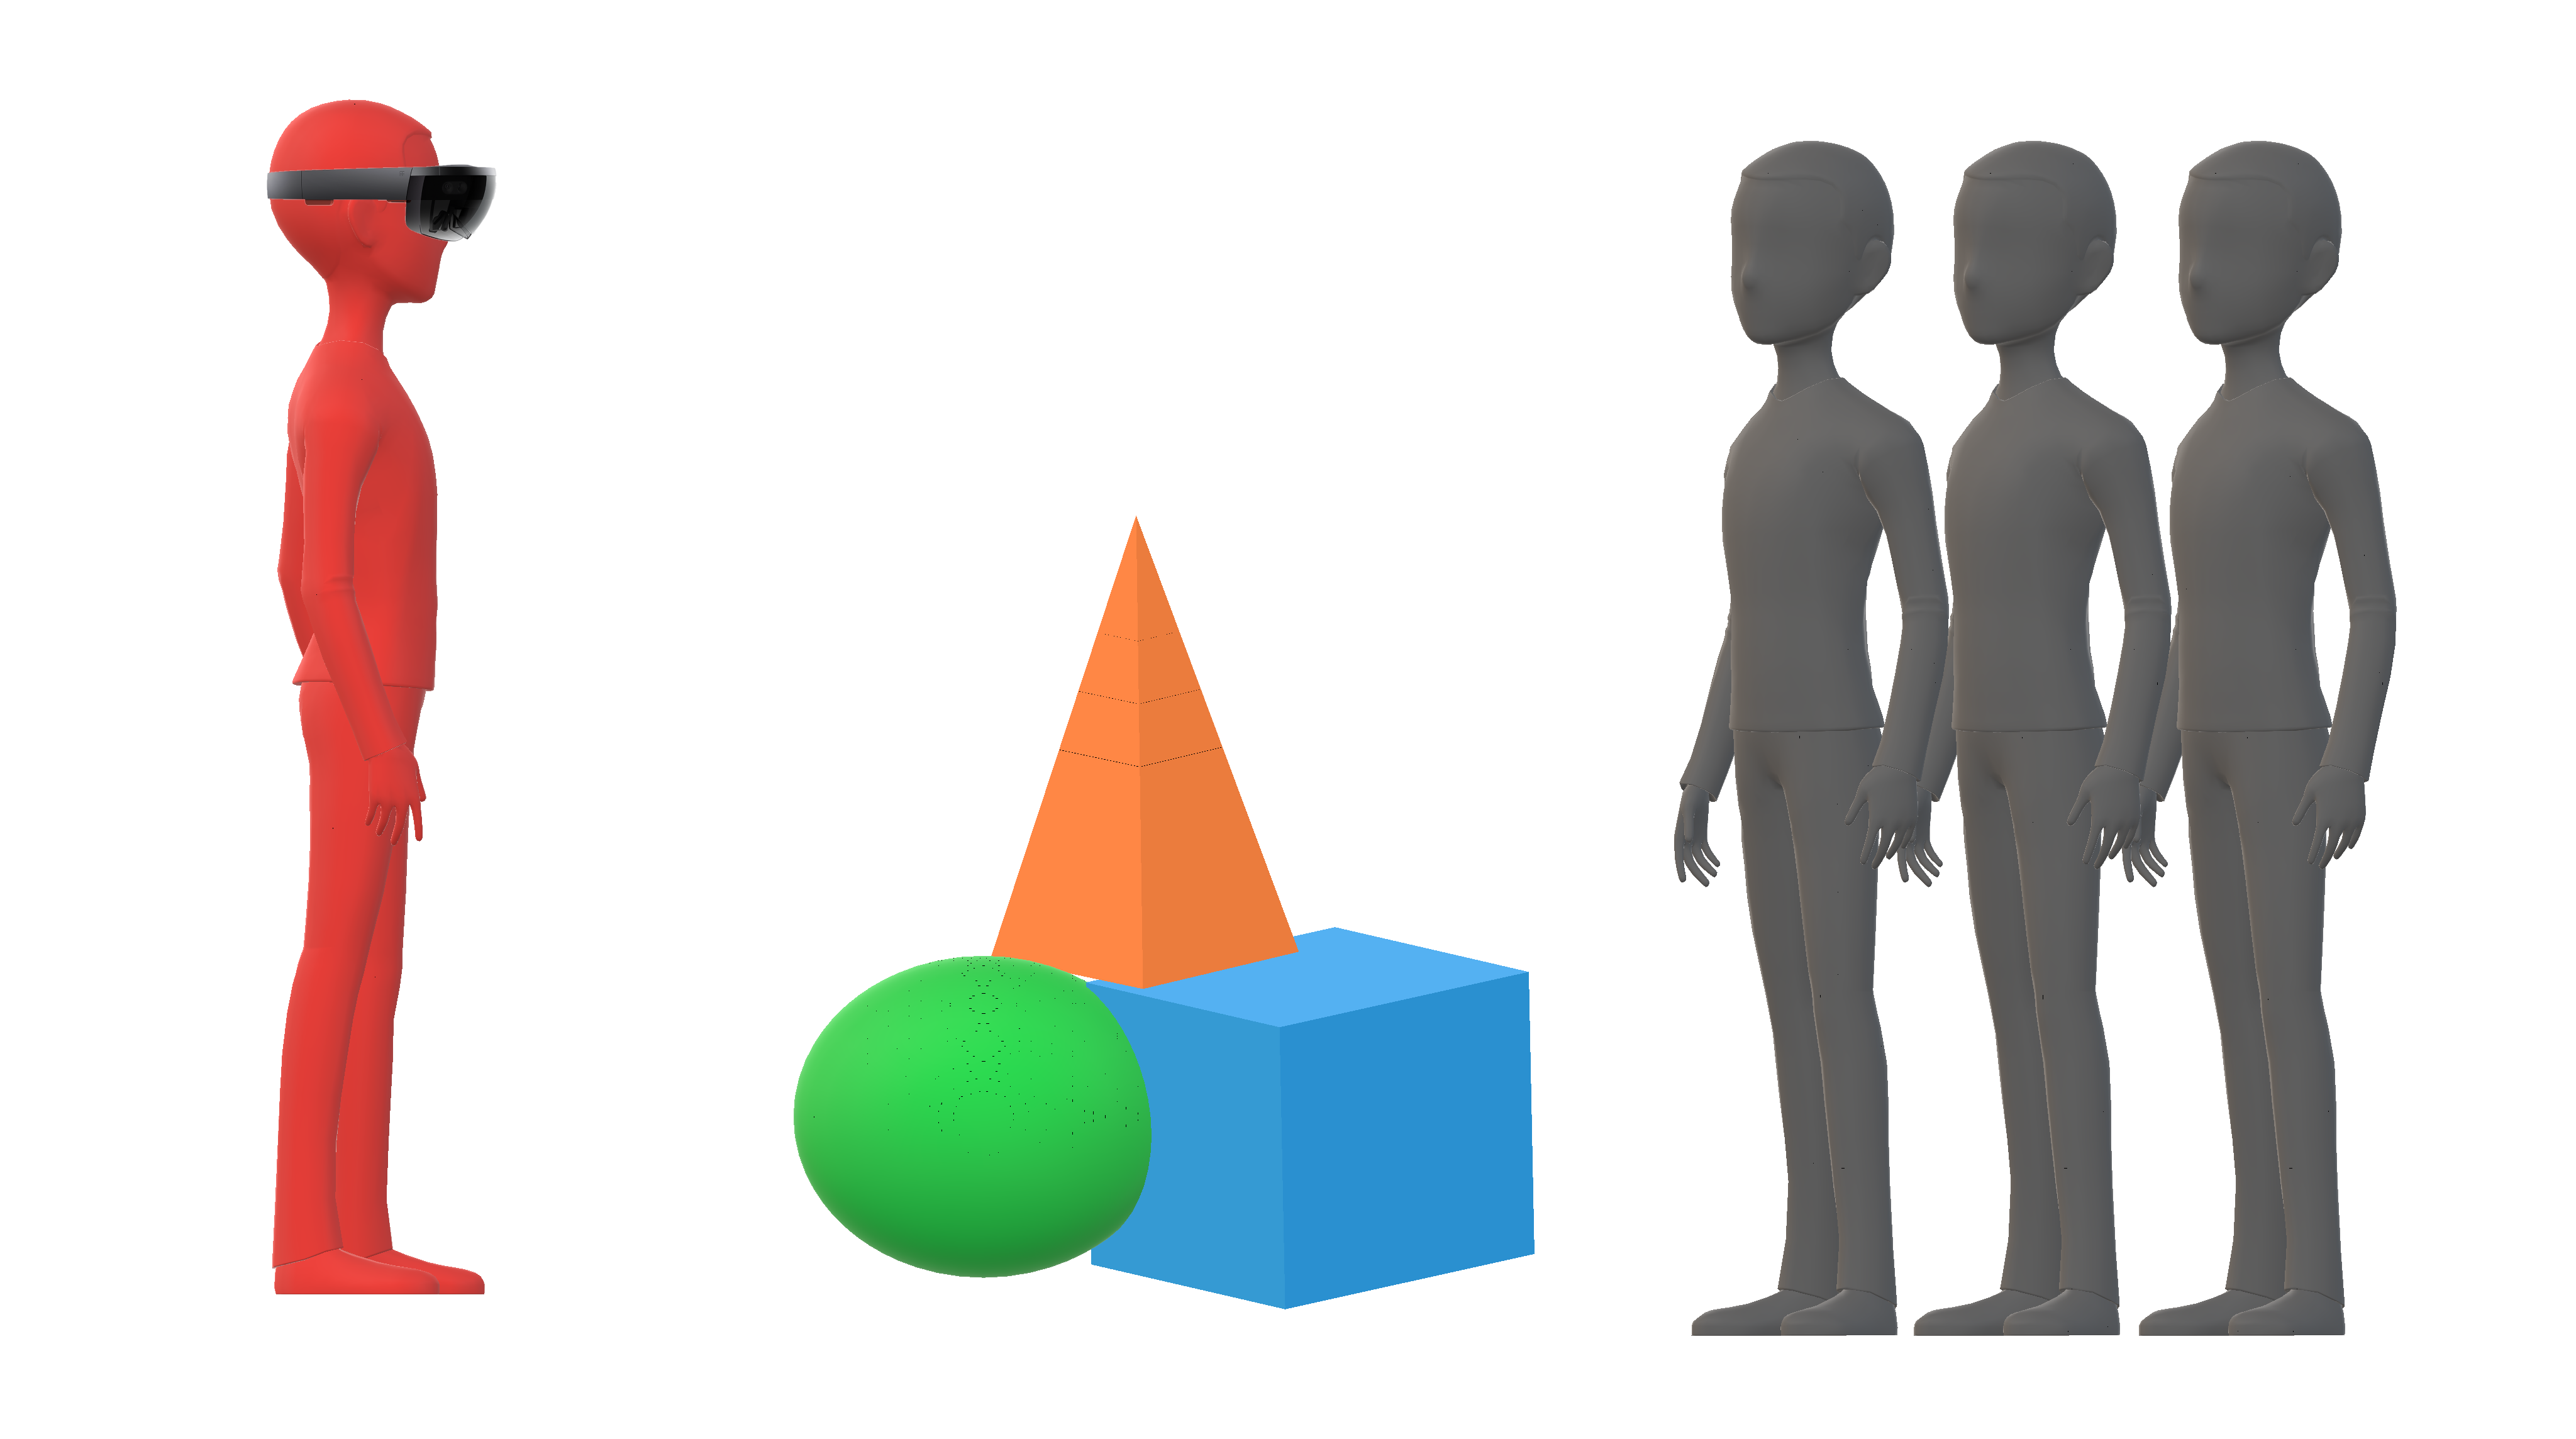
\includegraphics[width=0.8\linewidth]{images/30-continuum/continuum_categories5.png}
    \caption{The Social AR Continuum categories: 1) People (self and others), 2) Data \& objects (surrounding environment), 3) Interactions (e.g., annotations)}
    \label{fig:continuum:categories}
\end{figure}

This work categorises the social AR dimensions into three areas: 
\begin{enumerate}
    \item People (self and others) - a.k.a. \textit{social contacts},
    \item Data (including virtual objects and the surrounding environment), and
    \item Interactions between people and data (including annotation)
\end{enumerate}

Representing self and others as avatars is described in more detail in Chapter \ref{ch:contacts}. The surrounding environment and sharing different types of data are described in more detail in Chapter \ref{ch:data}, while the interactions between people, in the form of annotation of the surrounding environment, are described in Chapter \ref{ch:annotation}.

The Social AR Continuum varies based on the closeness of social connections that we have with others (our relationships), and this thesis identified the following dimensions where social AR applications can fit along a continuum. The dimensions can be grouped in the categories described in Figure \ref{fig:continuum:dimensions}.

\begin{figure}[ht]
    \centering
    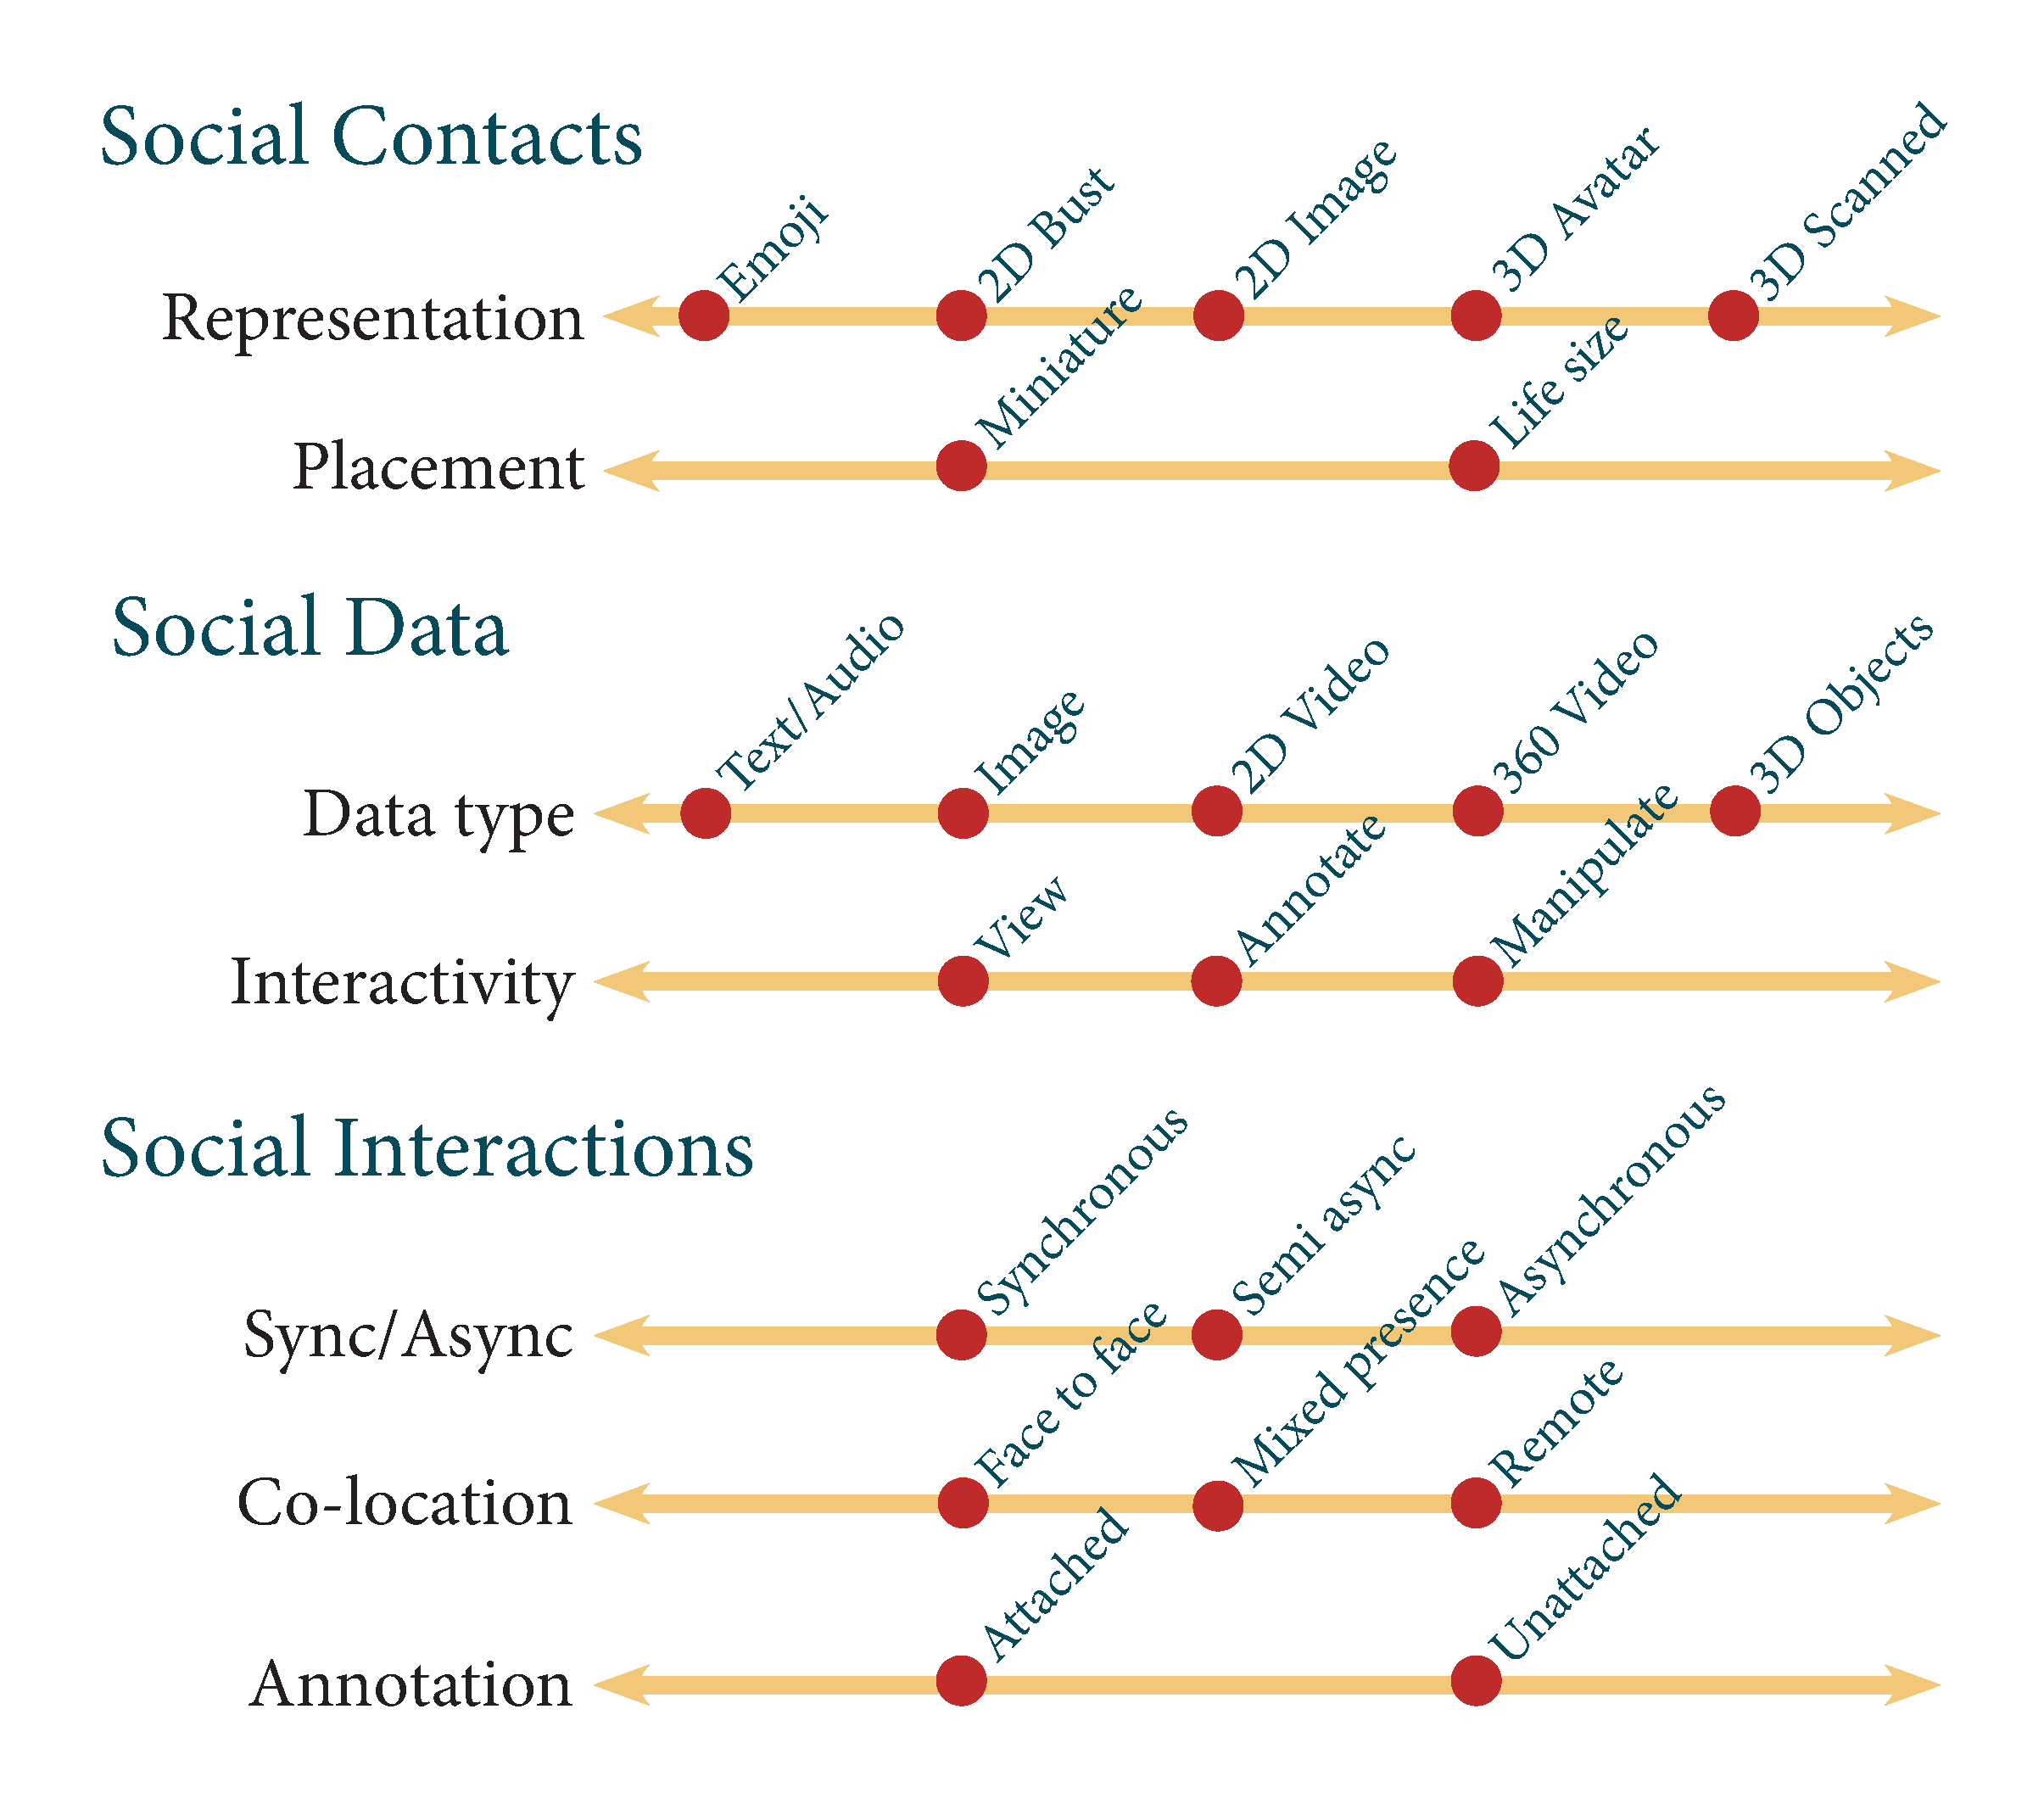
\includegraphics[width=\linewidth]{images/30-continuum/continuum43-01.eps}
    \caption{Dimensions of the Social AR Continuum.}
    \label{fig:continuum:dimensions}
\end{figure}

The definition of the dimensions of the Social AR Continuum has evolved during this research. It started (Figure \ref{fig:continuum:old-dimensions}) by merely looking at different configurations or options that can be changed when sharing social experiences on an AR headset. The original version focused on two types of social relationships: Friends and Strangers.

\begin{figure}[ht]
    \centering
    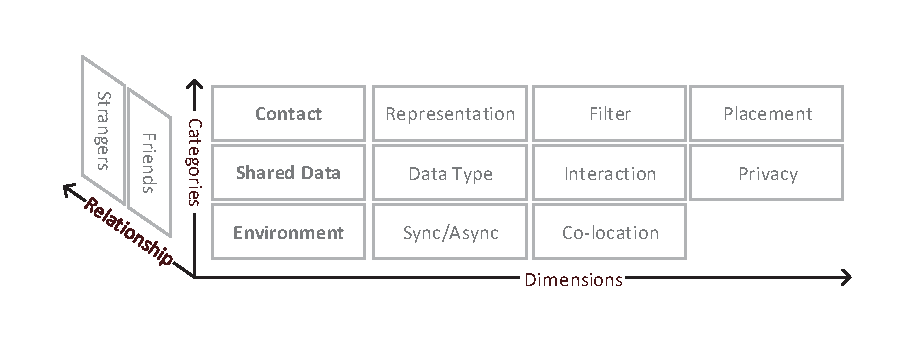
\includegraphics[width=\linewidth]{images/30-continuum/original-dimensions-diagram.eps}
    \caption{Earlier version of the dimensions of the Social AR Continuum.}
    \label{fig:continuum:old-dimensions}
\end{figure}

\subsection{Social Contact Representation}

In the social context, people are being referred to as \textit{social contacts} indicating that the user can get in touch with them for the purpose of sharing social experiences such as sharing a photo, sending a message, etc. Therefore the word \textit{contact} here is used to refer to a social friend. 

Representation of social contacts (Figure \ref{fig:continuum:contact-representations}) can vary on the Social AR Continuum based on the relationship that the user has with the contact, with closer relationships having a higher fidelity representation. For example, \textit{Intimate} contacts could be represented as full 3D animated avatars, \textit{Friends} could be represented as 2D static images, \textit{Acquaintances} could be represented as 2D busts and \textit{Strangers} could be shown as mere emojis. Each contact could choose their representation for each category.

\begin{figure}[ht]
    \centering
    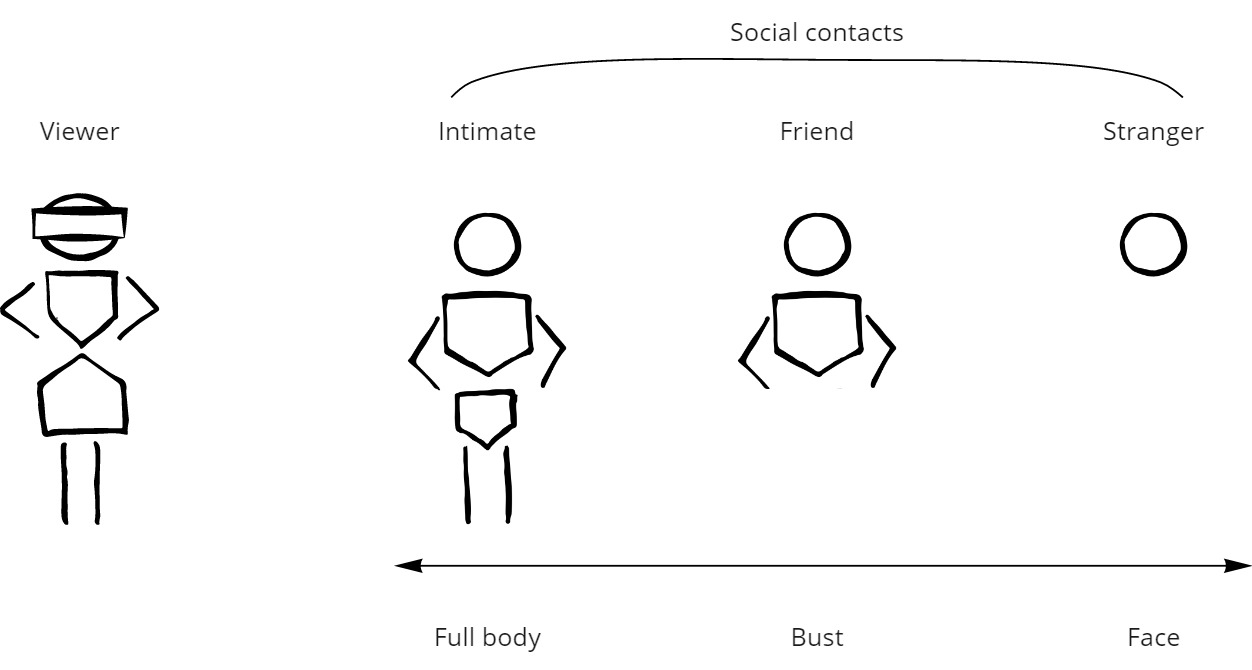
\includegraphics[width=0.8\linewidth]{images/30-continuum/Continuum-representation.jpg}
    \caption{Illustration of contact representations options based on social proximity. An intimate social contact appear in full body to the viewer, while a friend appear in upper half of the body as a 2D image. A stranger appears as an emoticon representing their face. (original icons from Noun Project \cite{TheNounProjectInc.})}
    \label{fig:continuum:contact-representations}
\end{figure}

% \textbf{Contact Filter}
% Filtering social contacts to distinguish users from each other could be done using proximity or visual fidelity based on their relationship to the user. Proximity filters contacts by placing them closer or further away. Visual fidelity filters contacts by adding more level of detail to the contact for closer relationships and less detail for further away contacts. 

\subsection{Social Contact Placement}

Placing social contacts (Figure \ref{fig:continuum:contact-placement}) can be done by displaying \textit{Intimates} as life-sized avatars on the ground around the user, and others as miniatures on a nearby surface. 

\begin{figure}[ht]
    \centering
    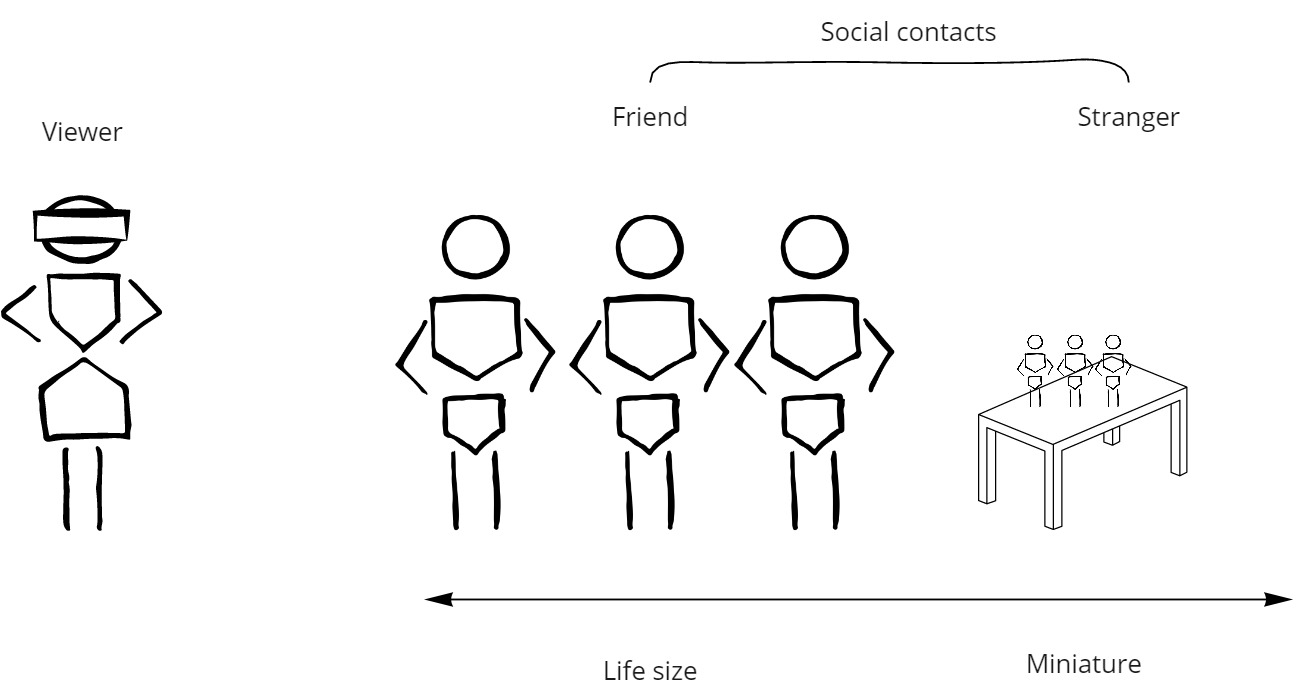
\includegraphics[width=0.8\linewidth]{images/30-continuum/Continuum-placement.jpg}
    \caption{Illustration of Contact placement options based on social proximity. Close friends can be displayed as life-size avatars, while other can be displayed as a miniature figures. (original icons from Noun Project \cite{TheNounProjectInc.})}
    \label{fig:continuum:contact-placement}
\end{figure}

% \subsection{Contact transparency}
% \todo[inline]{Add illustration}


% The transparency of social contacts can be used based on social proximity. Closer social contacts appear more opaque while further away ones appear more transparent.

\subsection{Data Type}

The type of data (Figure \ref{fig:continuum:data-type}) shared between social contacts in AR could be categorised as 1D (e.g., text or audio), 2D (e.g., images, panorama or video), or 3D (e.g., 3D model or scanned-room environment). Based on the relationship between the user and their social contacts, the type of data available could be filtered. For instance, 3D data could be shared with \textit{Intimate} relationships, while \textit{Acquaintances} could see only 2D data.  

\begin{figure}[ht]
    \centering
    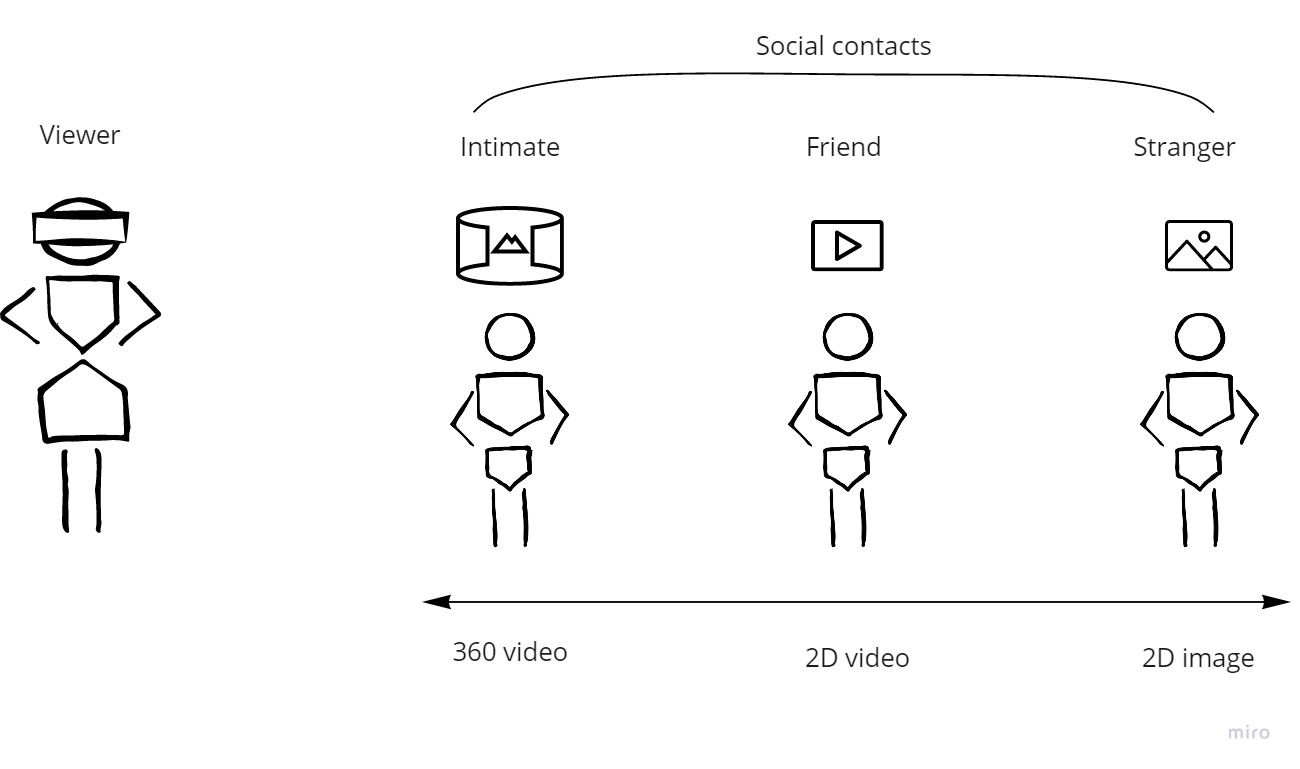
\includegraphics[width=0.8\linewidth]{images/30-continuum/Continuum-Data-type.jpg}
    \caption{Illustration of data type options. Close social contacts can see higher fidelity of shared data than the socially further away ones. (original icons from Noun Project \cite{TheNounProjectInc.})}
    \label{fig:continuum:data-type}
\end{figure}

\subsection{Data Interactivity}

In terms of user interactions (Figure \ref{fig:continuum:data-interaction}) with shared data, the Social AR Continuum here ranges from viewing the contents, annotating or adding comments on the content, through to manipulating the content. Levels of manipulation include changing the position, rotation or scale of the shared content, or even modifying the content itself.

\begin{figure}[ht]
    \centering
    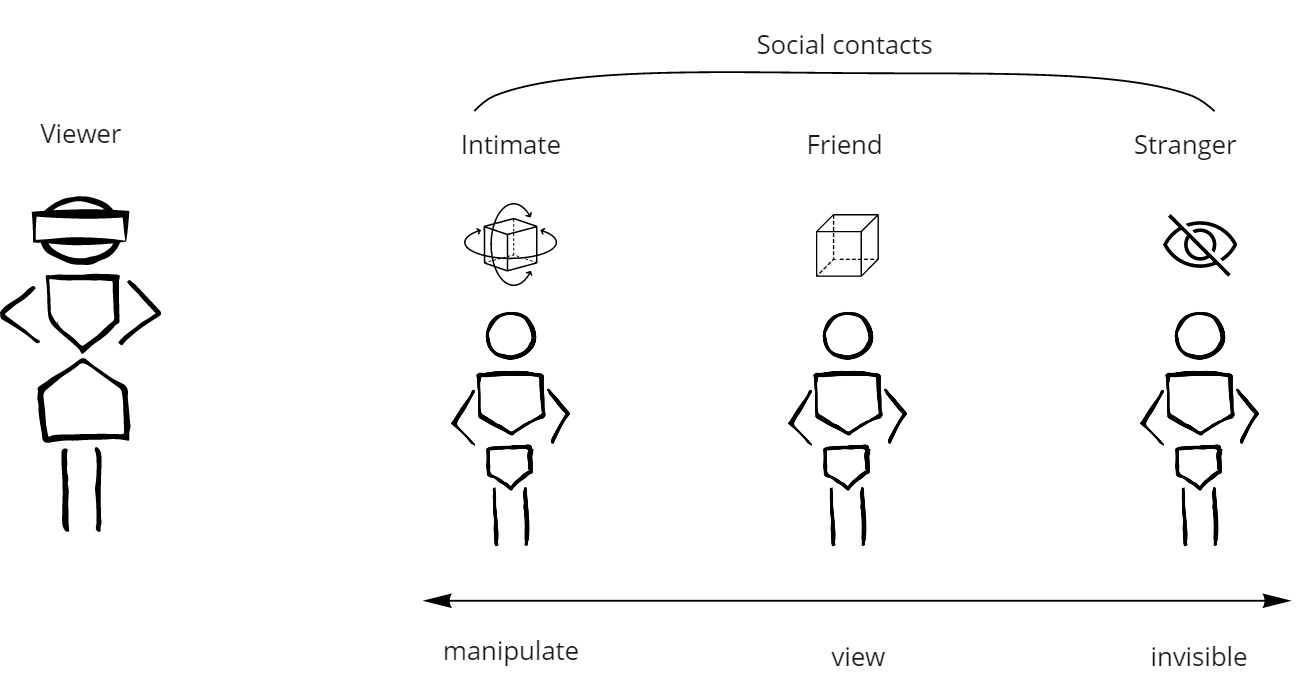
\includegraphics[width=0.8\linewidth]{images/30-continuum/Continuum-interaction.jpg}
    \caption{Illustration of data interactivity options. Closer social contacts can interact with the shared data in higher fidelity (add/edit/remote) than the further away ones (view only). (original icons from Noun Project \cite{TheNounProjectInc.})}
    \label{fig:continuum:data-interaction}
\end{figure}

% \subsection{Data Privacy}
% \todo[inline]{Add this to the dimensions figure}

% Based on the relationship with other users, shared data can be made private to the user, shared with specific groups of people (e.g., friends, acquaintances), or shared with everyone. This will allow users to choose the privacy levels of the shared data based on their social relationship with others. 

\subsection{Synchronous/Asynchronous Data}

The synchronicity of the shared data (Figure \ref{fig:continuum:data-connection}) can be represented based on social proximity. The data shared with contacts could be shared in a synchronous way, where both sharing and interaction happen at the same time. In contrast, data could also be shared asynchronously \cite{Smith2016}, i.e., interaction happens at a different time. 

\begin{figure}[ht]
    \centering
    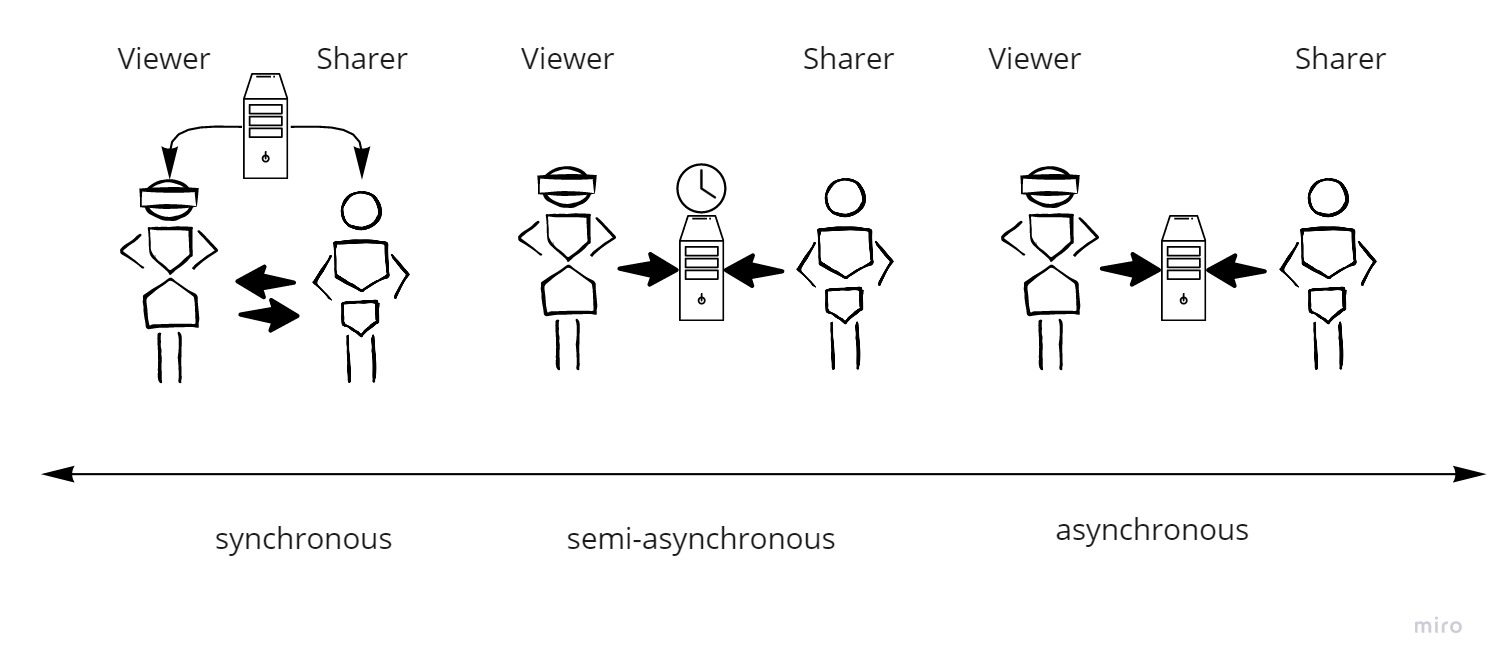
\includegraphics[width=0.8\linewidth]{images/30-continuum/continuum-connection.jpg}
    \caption{Illustration of data connection options. (original icons from Noun Project \cite{TheNounProjectInc.})}
    \label{fig:continuum:data-connection}
\end{figure}

\subsection{Co-location}

% \todo[inline]{Gun Lee: This sounds more generic concept in collaboration, rather than having social aspects. I.e. would colocation controlled/adjusted depending on social proximity as you do with other dimensions? Or would this be merely a description of collaborative scenarios?}

The co-location of the social contacts and their interactions (Figure \ref{fig:continuum:data-colocation}) can be represented based on social proximity. Options for representing social people or data can be in: 
1) remote (i.e., in a different place than the user), 
2) face-to-face (i.e., physically in the same location as the user), or 
3) semi face-to-face (i.e., where the social contact/data is physically in the same location, but virtually hidden or removed). When social contacts are remote, they are represented as virtual avatars based on their relationship with the user. When social contacts are face to face, then AR information is displayed attached to their body (i.e., when social contact moves, the information moves with them). 
An example of a semi face-to-face interaction was described in a Black Mirror\footnote{http://www.imdb.com/title/tt2085059/} episode "White Christmas" where a person could \textit{block} another co-located person by blurring them out in their AR view of the real world.

\begin{figure}[ht]
    \centering
    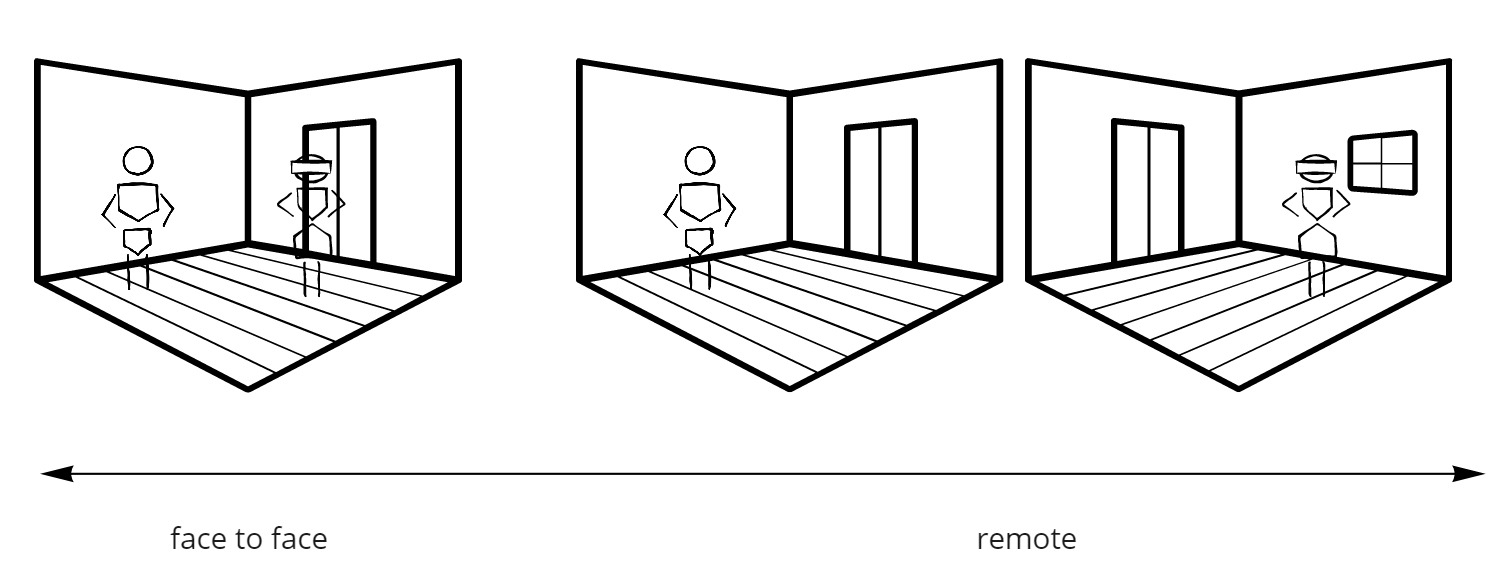
\includegraphics[width=0.8\linewidth]{images/30-continuum/continuum-colocation.jpg}
    \caption{Illustration of data co-location options. (original icons from Noun Project \cite{TheNounProjectInc.})}
    \label{fig:continuum:data-colocation}
\end{figure}

\subsection{Annotation}
% \todo[inline]{Add illustration}

Placing AR annotations (Figure \ref{fig:continuum:data-annotation}) or information attached to an AR object can be described as person/object-attached or not-attached. 
This is inspired by \textcite{Billinghurst1998} describing the options of the registration of information as head-stabilised, body-stabilised or world-stabilised. 
When adding text to describe an object or a place, the text can be placed as a list (lower fidelity) on the side of the screen or can be placed on the related object as an AR annotation (higher fidelity) that "sticks" to the scene and disappears if the user looks away. 
This dimension can be used with social contacts, and if the contact is a close friend, they would see the AR annotation in higher fidelity (attached to the person or the object), while a stranger would see the text annotations in lower fidelity (unattached to anything, but just as a list). 

% \todo[inline]{Rob: Seems odd. Do you mean they might see that there is an annotation , but can not read it?}

\begin{figure}[ht]
    \centering
    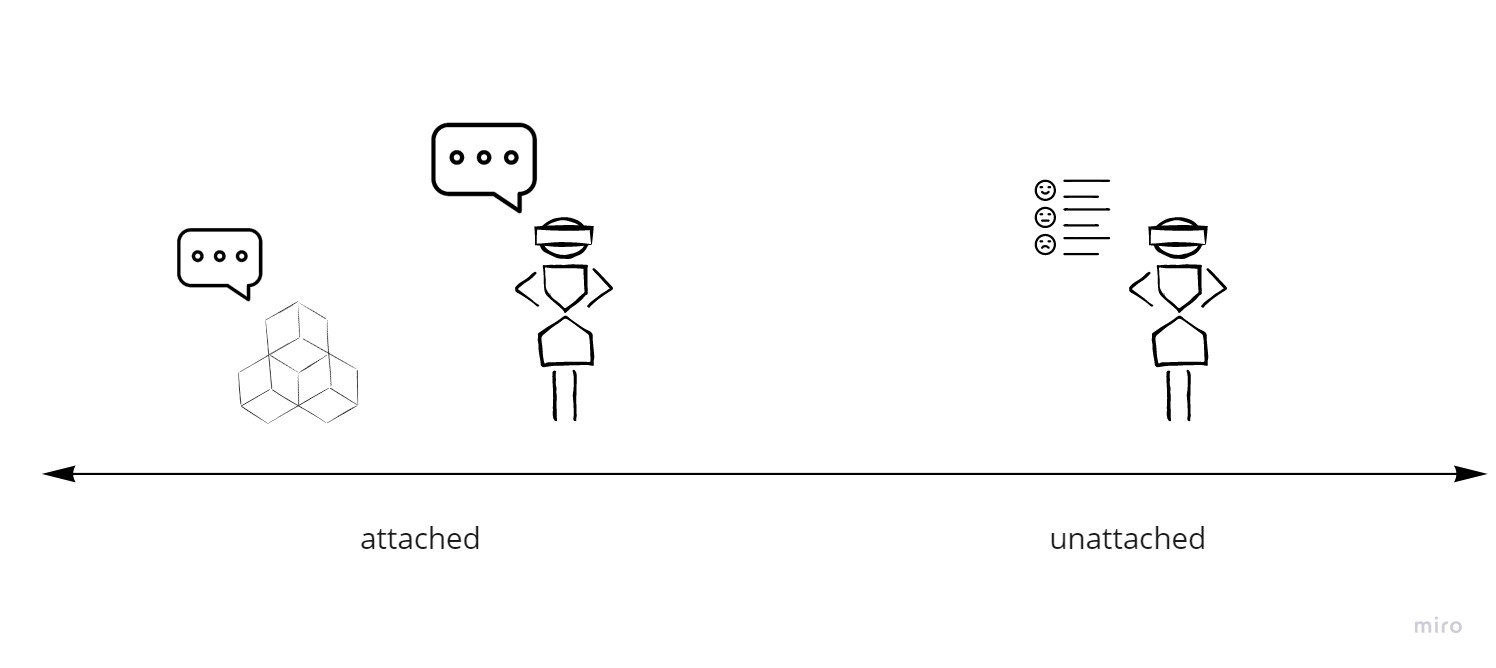
\includegraphics[width=0.8\linewidth]{images/30-continuum/continuum-annotation-2.jpg}
    \caption{Illustration of annotation options. (original icons from Noun Project \cite{TheNounProjectInc.})}
    \label{fig:continuum:data-annotation}
\end{figure}

% gogo: Another way to think about list vs. callouts is view-fixed (list) versus world-fixed (callouts). Feiner (I think it was him) defined a set of locations/things that text/windows could be attached to


% \subsection{Collaboration}
% When collaborating with social contacts, the user could use a pointer (e.g. arrow, indicator) to direct the conversation to a particular place or use a drawing tool (e.g. a pencil) to highlight the area of the conversation. The availability of these options could depend on the social proximity between social contacts. If closer to each other, higher fidelity tools are available, and if strangers, then the collaboration is limited to lower fidelity tools.

% \subsection{Awareness}

% It is possible during a session of sharing social experiences, that social contacts are looking in different directions. Awareness tools help users to know where the other user is looking. This can be achieved by showing a rectangle or a circle pointing to where the user is looking, or by using a context compass view which provides higher fidelity for closer connections.

% Gun: add a bit more details on how controlling each dimension based on social proximity would benefit

\section{Summary}

This work introduced the concept of the Social AR Continuum and identified several dimensions where a social AR application could be implemented.

3D avatar not always better than 2D. 360 video not always better than 2D image. If different content or more focused content can be useful in lower fidelity, but if the same data/content is represented in 3D it will contain more details about the content than if it was only 2D. However, there is a downside of more content that can be overwhelming to the viewer. 

In the future, there will be additional dimensions on the AR continuum that can be added as guidelines. Social systems are driven by lots of users using them. This thesis focused on exploration of what a social system in AR would look like. After implementing such system and wide adoption, there will be other dimensions discovered. However, the general guidelines of representing people, data and interactions may not change completely. For instance, the hashtag concept was introduced by users of social networks, then later was adopted by social networks systems. 

The next chapters explores three categories on the Social AR Continuum through system prototypes and user studies.

% Gun: close this chapter by giving an overview of the next few chapters.